% Options for packages loaded elsewhere
\PassOptionsToPackage{unicode}{hyperref}
\PassOptionsToPackage{hyphens}{url}
%
\documentclass[
]{article}
\usepackage{amsmath,amssymb}
\usepackage{lmodern}
\usepackage{ifxetex,ifluatex}
\ifnum 0\ifxetex 1\fi\ifluatex 1\fi=0 % if pdftex
  \usepackage[T1]{fontenc}
  \usepackage[utf8]{inputenc}
  \usepackage{textcomp} % provide euro and other symbols
\else % if luatex or xetex
  \usepackage{unicode-math}
  \defaultfontfeatures{Scale=MatchLowercase}
  \defaultfontfeatures[\rmfamily]{Ligatures=TeX,Scale=1}
\fi
% Use upquote if available, for straight quotes in verbatim environments
\IfFileExists{upquote.sty}{\usepackage{upquote}}{}
\IfFileExists{microtype.sty}{% use microtype if available
  \usepackage[]{microtype}
  \UseMicrotypeSet[protrusion]{basicmath} % disable protrusion for tt fonts
}{}
\makeatletter
\@ifundefined{KOMAClassName}{% if non-KOMA class
  \IfFileExists{parskip.sty}{%
    \usepackage{parskip}
  }{% else
    \setlength{\parindent}{0pt}
    \setlength{\parskip}{6pt plus 2pt minus 1pt}}
}{% if KOMA class
  \KOMAoptions{parskip=half}}
\makeatother
\usepackage{xcolor}
\IfFileExists{xurl.sty}{\usepackage{xurl}}{} % add URL line breaks if available
\IfFileExists{bookmark.sty}{\usepackage{bookmark}}{\usepackage{hyperref}}
\hypersetup{
  pdftitle={R scripts can be rendered!},
  pdfauthor={Stefan Veleski},
  hidelinks,
  pdfcreator={LaTeX via pandoc}}
\urlstyle{same} % disable monospaced font for URLs
\usepackage[margin=1in]{geometry}
\usepackage{color}
\usepackage{fancyvrb}
\newcommand{\VerbBar}{|}
\newcommand{\VERB}{\Verb[commandchars=\\\{\}]}
\DefineVerbatimEnvironment{Highlighting}{Verbatim}{commandchars=\\\{\}}
% Add ',fontsize=\small' for more characters per line
\usepackage{framed}
\definecolor{shadecolor}{RGB}{248,248,248}
\newenvironment{Shaded}{\begin{snugshade}}{\end{snugshade}}
\newcommand{\AlertTok}[1]{\textcolor[rgb]{0.94,0.16,0.16}{#1}}
\newcommand{\AnnotationTok}[1]{\textcolor[rgb]{0.56,0.35,0.01}{\textbf{\textit{#1}}}}
\newcommand{\AttributeTok}[1]{\textcolor[rgb]{0.77,0.63,0.00}{#1}}
\newcommand{\BaseNTok}[1]{\textcolor[rgb]{0.00,0.00,0.81}{#1}}
\newcommand{\BuiltInTok}[1]{#1}
\newcommand{\CharTok}[1]{\textcolor[rgb]{0.31,0.60,0.02}{#1}}
\newcommand{\CommentTok}[1]{\textcolor[rgb]{0.56,0.35,0.01}{\textit{#1}}}
\newcommand{\CommentVarTok}[1]{\textcolor[rgb]{0.56,0.35,0.01}{\textbf{\textit{#1}}}}
\newcommand{\ConstantTok}[1]{\textcolor[rgb]{0.00,0.00,0.00}{#1}}
\newcommand{\ControlFlowTok}[1]{\textcolor[rgb]{0.13,0.29,0.53}{\textbf{#1}}}
\newcommand{\DataTypeTok}[1]{\textcolor[rgb]{0.13,0.29,0.53}{#1}}
\newcommand{\DecValTok}[1]{\textcolor[rgb]{0.00,0.00,0.81}{#1}}
\newcommand{\DocumentationTok}[1]{\textcolor[rgb]{0.56,0.35,0.01}{\textbf{\textit{#1}}}}
\newcommand{\ErrorTok}[1]{\textcolor[rgb]{0.64,0.00,0.00}{\textbf{#1}}}
\newcommand{\ExtensionTok}[1]{#1}
\newcommand{\FloatTok}[1]{\textcolor[rgb]{0.00,0.00,0.81}{#1}}
\newcommand{\FunctionTok}[1]{\textcolor[rgb]{0.00,0.00,0.00}{#1}}
\newcommand{\ImportTok}[1]{#1}
\newcommand{\InformationTok}[1]{\textcolor[rgb]{0.56,0.35,0.01}{\textbf{\textit{#1}}}}
\newcommand{\KeywordTok}[1]{\textcolor[rgb]{0.13,0.29,0.53}{\textbf{#1}}}
\newcommand{\NormalTok}[1]{#1}
\newcommand{\OperatorTok}[1]{\textcolor[rgb]{0.81,0.36,0.00}{\textbf{#1}}}
\newcommand{\OtherTok}[1]{\textcolor[rgb]{0.56,0.35,0.01}{#1}}
\newcommand{\PreprocessorTok}[1]{\textcolor[rgb]{0.56,0.35,0.01}{\textit{#1}}}
\newcommand{\RegionMarkerTok}[1]{#1}
\newcommand{\SpecialCharTok}[1]{\textcolor[rgb]{0.00,0.00,0.00}{#1}}
\newcommand{\SpecialStringTok}[1]{\textcolor[rgb]{0.31,0.60,0.02}{#1}}
\newcommand{\StringTok}[1]{\textcolor[rgb]{0.31,0.60,0.02}{#1}}
\newcommand{\VariableTok}[1]{\textcolor[rgb]{0.00,0.00,0.00}{#1}}
\newcommand{\VerbatimStringTok}[1]{\textcolor[rgb]{0.31,0.60,0.02}{#1}}
\newcommand{\WarningTok}[1]{\textcolor[rgb]{0.56,0.35,0.01}{\textbf{\textit{#1}}}}
\usepackage{graphicx}
\makeatletter
\def\maxwidth{\ifdim\Gin@nat@width>\linewidth\linewidth\else\Gin@nat@width\fi}
\def\maxheight{\ifdim\Gin@nat@height>\textheight\textheight\else\Gin@nat@height\fi}
\makeatother
% Scale images if necessary, so that they will not overflow the page
% margins by default, and it is still possible to overwrite the defaults
% using explicit options in \includegraphics[width, height, ...]{}
\setkeys{Gin}{width=\maxwidth,height=\maxheight,keepaspectratio}
% Set default figure placement to htbp
\makeatletter
\def\fps@figure{htbp}
\makeatother
\setlength{\emergencystretch}{3em} % prevent overfull lines
\providecommand{\tightlist}{%
  \setlength{\itemsep}{0pt}\setlength{\parskip}{0pt}}
\setcounter{secnumdepth}{-\maxdimen} % remove section numbering
\ifluatex
  \usepackage{selnolig}  % disable illegal ligatures
\fi

\title{R scripts can be rendered!}
\author{Stefan Veleski}
\date{May 13, 2021}

\begin{document}
\maketitle

Tidytext sentiment analysis Loading in the necessary packages

\begin{Shaded}
\begin{Highlighting}[]
\FunctionTok{library}\NormalTok{(tidyverse)}
\FunctionTok{library}\NormalTok{(syuzhet)}
\FunctionTok{library}\NormalTok{(gutenbergr)}
\FunctionTok{library}\NormalTok{(tidytext)}
\FunctionTok{library}\NormalTok{(textdata)}
\end{Highlighting}
\end{Shaded}

\begin{Shaded}
\begin{Highlighting}[]
\NormalTok{hardy\_meta }\OtherTok{\textless{}{-}} \FunctionTok{gutenberg\_works}\NormalTok{(author }\SpecialCharTok{==} \StringTok{"Hardy, Thomas"}\NormalTok{) }\CommentTok{\# Download metadata for Hardy\textquotesingle{}s works}
\NormalTok{hardy\_meta }\OtherTok{\textless{}{-}}\NormalTok{ hardy\_meta }\SpecialCharTok{\%\textgreater{}\%} 
  \FunctionTok{slice}\NormalTok{(}\FunctionTok{c}\NormalTok{(}\DecValTok{1}\NormalTok{,}\DecValTok{2}\NormalTok{,}\DecValTok{3}\NormalTok{,}\DecValTok{4}\NormalTok{,}\DecValTok{5}\NormalTok{,}\DecValTok{6}\NormalTok{,}\DecValTok{7}\NormalTok{,}\DecValTok{8}\NormalTok{,}\DecValTok{10}\NormalTok{,}\DecValTok{11}\NormalTok{,}\DecValTok{13}\NormalTok{,}\DecValTok{18}\NormalTok{,}\DecValTok{22}\NormalTok{,}\DecValTok{23}\NormalTok{,}\DecValTok{24}\NormalTok{)) }\CommentTok{\# Manually selecting Hardy\textquotesingle{}s novels}
\end{Highlighting}
\end{Shaded}

\begin{Shaded}
\begin{Highlighting}[]
\NormalTok{austen\_meta }\OtherTok{\textless{}{-}} \FunctionTok{gutenberg\_works}\NormalTok{(author }\SpecialCharTok{==} \StringTok{"Austen, Jane"}\NormalTok{) }\CommentTok{\# Download metadata for Austen\textquotesingle{}s works}
\NormalTok{austen\_meta }\OtherTok{\textless{}{-}}\NormalTok{ austen\_meta }\SpecialCharTok{\%\textgreater{}\%}  \CommentTok{\# Cutting off two compilation works that are not necessary }
  \FunctionTok{slice}\NormalTok{(}\DecValTok{1}\SpecialCharTok{:}\DecValTok{8}\NormalTok{)}
\end{Highlighting}
\end{Shaded}

Download all of Hardy's and Austen's texts - retain a column with the
titles of the novels

\begin{Shaded}
\begin{Highlighting}[]
\NormalTok{hardy\_tidy\_texts }\OtherTok{\textless{}{-}} \FunctionTok{gutenberg\_download}\NormalTok{(hardy\_meta}\SpecialCharTok{$}\NormalTok{gutenberg\_id, }
                                  \AttributeTok{meta\_fields =} \StringTok{"title"}\NormalTok{) }

\NormalTok{austen\_tidy\_texts }\OtherTok{\textless{}{-}} \FunctionTok{gutenberg\_download}\NormalTok{(austen\_meta}\SpecialCharTok{$}\NormalTok{gutenberg\_id,}
                                  \AttributeTok{meta\_fields =} \StringTok{"title"}\NormalTok{)}
\end{Highlighting}
\end{Shaded}

The following code tokenizes the full text by individual words, but also
provides additional metadata about the line and the chapter that the
word is located in

\begin{Shaded}
\begin{Highlighting}[]
\NormalTok{austen\_tidy\_texts }\OtherTok{\textless{}{-}}\NormalTok{ austen\_tidy\_texts }\SpecialCharTok{\%\textgreater{}\%}
  \FunctionTok{group\_by}\NormalTok{(title) }\SpecialCharTok{\%\textgreater{}\%}
  \FunctionTok{mutate}\NormalTok{(}
    \AttributeTok{linenumber =} \FunctionTok{row\_number}\NormalTok{(),}
    \AttributeTok{chapter =} \FunctionTok{cumsum}\NormalTok{(}\FunctionTok{str\_detect}\NormalTok{(text,  }\CommentTok{\#cumulative sum, detect string, column analyzed}
                                \FunctionTok{regex}\NormalTok{(}\StringTok{"\^{}chapter [}\SpecialCharTok{\textbackslash{}\textbackslash{}}\StringTok{divxlc]"}\NormalTok{, }\CommentTok{\# regular expression, chapter any char}
                                      \AttributeTok{ignore\_case =} \ConstantTok{TRUE}\NormalTok{)))) }\SpecialCharTok{\%\textgreater{}\%} \CommentTok{\# include both lower and uppercase}
  \FunctionTok{ungroup}\NormalTok{() }\SpecialCharTok{\%\textgreater{}\%} \CommentTok{\# removing the grouping by title set up above}
  \FunctionTok{unnest\_tokens}\NormalTok{(word, text) }\CommentTok{\# tokenization of the text column by word (word per row)}

\NormalTok{nrc\_joy }\OtherTok{\textless{}{-}} \FunctionTok{get\_sentiments}\NormalTok{(}\StringTok{"nrc"}\NormalTok{) }\SpecialCharTok{\%\textgreater{}\%} \CommentTok{\# tidy text function that extracts the values of 3 sentiment lexicons}
  \FunctionTok{filter}\NormalTok{(sentiment }\SpecialCharTok{==} \StringTok{"joy"}\NormalTok{) }\CommentTok{\# filtering only joy}
\end{Highlighting}
\end{Shaded}

The ``Text Mining With R'' book uses the janeaustenr package, which is
not really

\begin{Shaded}
\begin{Highlighting}[]
\CommentTok{\# necessary, as we can represent the full workflow from downloading}
\CommentTok{\# the books to visualization, which can be used with books from other authors as well.}
\end{Highlighting}
\end{Shaded}

The code below simply counts the most common words in Persuasion that
correspond to the joy

\begin{Shaded}
\begin{Highlighting}[]
\CommentTok{\# emotion in the NRC sentiment lexicon}
\end{Highlighting}
\end{Shaded}

\begin{Shaded}
\begin{Highlighting}[]
\NormalTok{austen\_tidy\_texts }\SpecialCharTok{\%\textgreater{}\%}
  \FunctionTok{filter}\NormalTok{(title }\SpecialCharTok{==} \StringTok{"Persuasion"}\NormalTok{) }\SpecialCharTok{\%\textgreater{}\%} \CommentTok{\# only selecting Persuasion from the rest of the books}
  \FunctionTok{inner\_join}\NormalTok{(nrc\_joy) }\SpecialCharTok{\%\textgreater{}\%} \CommentTok{\# combining two tables together (see data wrangling cheat sheet)}
  \FunctionTok{count}\NormalTok{(word, }\AttributeTok{sort =} \ConstantTok{TRUE}\NormalTok{) }\CommentTok{\# counting the words}
\end{Highlighting}
\end{Shaded}

\begin{verbatim}
## # A tibble: 258 x 2
##    word        n
##    <chr>   <int>
##  1 good      187
##  2 young      84
##  3 found      83
##  4 friend     77
##  5 present    65
##  6 happy      64
##  7 hope       53
##  8 deal       45
##  9 love       42
## 10 spirits    41
## # ... with 248 more rows
\end{verbatim}

\begin{Shaded}
\begin{Highlighting}[]
\NormalTok{jane\_austen\_sentiment }\OtherTok{\textless{}{-}}\NormalTok{ austen\_tidy\_texts }\SpecialCharTok{\%\textgreater{}\%}
  \FunctionTok{inner\_join}\NormalTok{(}\FunctionTok{get\_sentiments}\NormalTok{(}\StringTok{"bing"}\NormalTok{)) }\SpecialCharTok{\%\textgreater{}\%} \CommentTok{\# change th}
  \FunctionTok{count}\NormalTok{(title, }\AttributeTok{index =}\NormalTok{ linenumber }\SpecialCharTok{\%/\%} \DecValTok{80}\NormalTok{, sentiment) }\SpecialCharTok{\%\textgreater{}\%}
  \FunctionTok{pivot\_wider}\NormalTok{(}\AttributeTok{names\_from =}\NormalTok{ sentiment, }\AttributeTok{values\_from =}\NormalTok{ n, }\AttributeTok{values\_fill =} \DecValTok{0}\NormalTok{) }\SpecialCharTok{\%\textgreater{}\%} 
  \FunctionTok{mutate}\NormalTok{(}\AttributeTok{sentiment =}\NormalTok{ positive }\SpecialCharTok{{-}}\NormalTok{ negative)}

\FunctionTok{ggplot}\NormalTok{(jane\_austen\_sentiment, }\FunctionTok{aes}\NormalTok{(index, sentiment, }\AttributeTok{fill =}\NormalTok{ title)) }\SpecialCharTok{+}
  \FunctionTok{geom\_col}\NormalTok{(}\AttributeTok{show.legend =} \ConstantTok{FALSE}\NormalTok{) }\SpecialCharTok{+}
  \FunctionTok{facet\_wrap}\NormalTok{(}\SpecialCharTok{\textasciitilde{}}\NormalTok{title, }\AttributeTok{ncol =} \DecValTok{2}\NormalTok{, }\AttributeTok{scales =} \StringTok{"free\_x"}\NormalTok{)}
\end{Highlighting}
\end{Shaded}

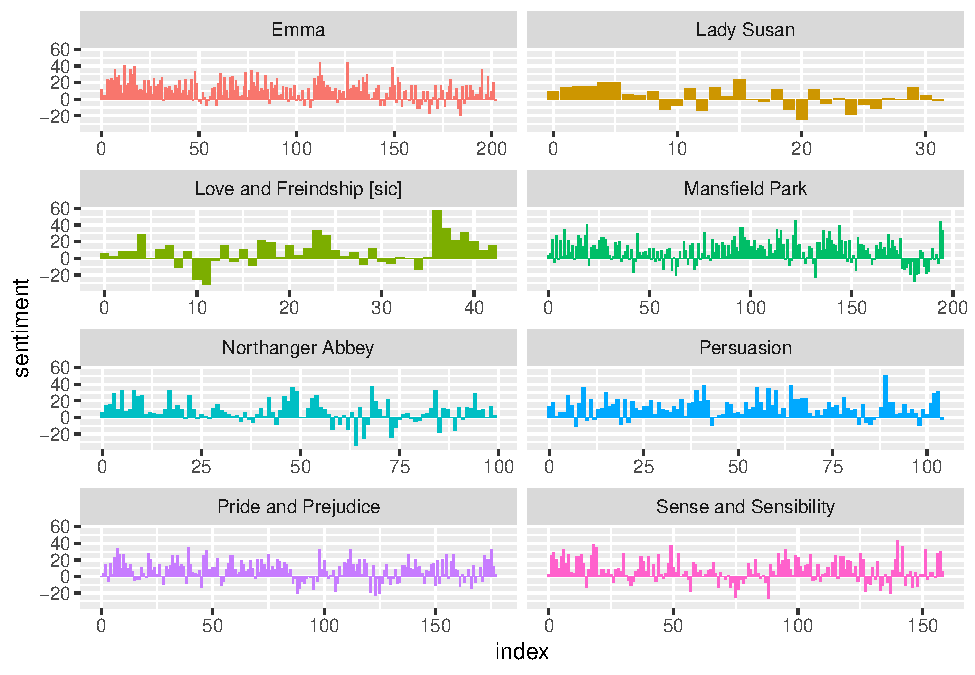
\includegraphics{Week8_files/figure-latex/unnamed-chunk-8-1.pdf}

Most common positive and negative words

\begin{Shaded}
\begin{Highlighting}[]
\NormalTok{bing\_word\_counts }\OtherTok{\textless{}{-}}\NormalTok{ austen\_tidy\_texts }\SpecialCharTok{\%\textgreater{}\%}
  \FunctionTok{inner\_join}\NormalTok{(}\FunctionTok{get\_sentiments}\NormalTok{(}\StringTok{"bing"}\NormalTok{)) }\SpecialCharTok{\%\textgreater{}\%} \CommentTok{\#retain only words that exist in both }
  \FunctionTok{count}\NormalTok{(word, sentiment, }\AttributeTok{sort =} \ConstantTok{TRUE}\NormalTok{) }\SpecialCharTok{\%\textgreater{}\%} 
  \FunctionTok{ungroup}\NormalTok{()}

\NormalTok{bing\_word\_counts }\SpecialCharTok{\%\textgreater{}\%}
  \FunctionTok{group\_by}\NormalTok{(sentiment) }\SpecialCharTok{\%\textgreater{}\%}
  \FunctionTok{slice\_max}\NormalTok{(n, }\AttributeTok{n =} \DecValTok{10}\NormalTok{) }\SpecialCharTok{\%\textgreater{}\%}  \CommentTok{\# slice n to retain top 10}
  \FunctionTok{ungroup}\NormalTok{() }\SpecialCharTok{\%\textgreater{}\%}
  \FunctionTok{mutate}\NormalTok{(}\AttributeTok{word =} \FunctionTok{reorder}\NormalTok{(word, n)) }\SpecialCharTok{\%\textgreater{}\%}
  \FunctionTok{ggplot}\NormalTok{(}\FunctionTok{aes}\NormalTok{(n, word, }\AttributeTok{fill =}\NormalTok{ sentiment)) }\SpecialCharTok{+} \CommentTok{\# n x axis, word y axis, color according to sentiment}
  \FunctionTok{geom\_col}\NormalTok{(}\AttributeTok{show.legend =} \ConstantTok{FALSE}\NormalTok{) }\SpecialCharTok{+} \CommentTok{\# barplot, no legends}
  \FunctionTok{facet\_wrap}\NormalTok{(}\SpecialCharTok{\textasciitilde{}}\NormalTok{sentiment, }\AttributeTok{scales =} \StringTok{"free\_y"}\NormalTok{) }\SpecialCharTok{+} \CommentTok{\# facet wrapped along sentiment, free y scale}
  \FunctionTok{labs}\NormalTok{(}\AttributeTok{x =} \StringTok{"Contribution to sentiment"}\NormalTok{, }\CommentTok{\# x label}
       \AttributeTok{y =} \ConstantTok{NULL}\NormalTok{) }\CommentTok{\# no y label}
\end{Highlighting}
\end{Shaded}

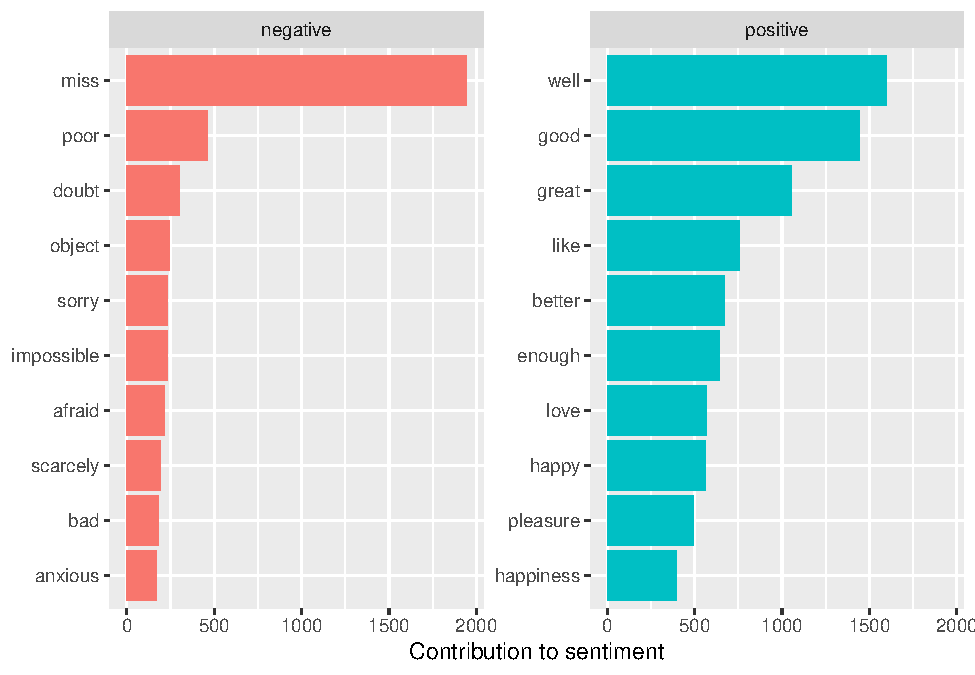
\includegraphics{Week8_files/figure-latex/unnamed-chunk-9-1.pdf}

\begin{Shaded}
\begin{Highlighting}[]
\CommentTok{\# Export in 5x10}
\end{Highlighting}
\end{Shaded}

Adding miss as a custom stopword to the stopwords lexicon contained in
the tidytext package. This will be removed from the visualization later
on

\begin{Shaded}
\begin{Highlighting}[]
\NormalTok{custom\_stop\_words }\OtherTok{\textless{}{-}} \FunctionTok{bind\_rows}\NormalTok{(}\FunctionTok{tibble}\NormalTok{(}\AttributeTok{word =} \FunctionTok{c}\NormalTok{(}\StringTok{"miss"}\NormalTok{),  }
                                      \AttributeTok{lexicon =} \FunctionTok{c}\NormalTok{(}\StringTok{"custom"}\NormalTok{)), }
\NormalTok{                               stop\_words)}
\end{Highlighting}
\end{Shaded}

Wordclouds clear plot cache

\begin{Shaded}
\begin{Highlighting}[]
\FunctionTok{library}\NormalTok{(wordcloud)}
\end{Highlighting}
\end{Shaded}

\begin{verbatim}
## Loading required package: RColorBrewer
\end{verbatim}

\begin{Shaded}
\begin{Highlighting}[]
\FunctionTok{library}\NormalTok{(reshape2)}
\end{Highlighting}
\end{Shaded}

\begin{verbatim}
## 
## Attaching package: 'reshape2'
\end{verbatim}

\begin{verbatim}
## The following object is masked from 'package:tidyr':
## 
##     smiths
\end{verbatim}

\begin{Shaded}
\begin{Highlighting}[]
\FunctionTok{set.seed}\NormalTok{(}\DecValTok{1234}\NormalTok{) }\CommentTok{\# reproducibility}
\NormalTok{austen\_tidy\_texts }\SpecialCharTok{\%\textgreater{}\%}
  \FunctionTok{anti\_join}\NormalTok{(custom\_stop\_words) }\SpecialCharTok{\%\textgreater{}\%} \CommentTok{\# remove all words that have a match in custom\_stop\_words}
  \FunctionTok{inner\_join}\NormalTok{(}\FunctionTok{get\_sentiments}\NormalTok{(}\StringTok{"bing"}\NormalTok{)) }\SpecialCharTok{\%\textgreater{}\%} \CommentTok{\# retain only words that exist in both }
  \FunctionTok{count}\NormalTok{(word, sentiment, }\AttributeTok{sort =} \ConstantTok{TRUE}\NormalTok{) }\SpecialCharTok{\%\textgreater{}\%} \CommentTok{\#}
  \FunctionTok{acast}\NormalTok{(word }\SpecialCharTok{\textasciitilde{}}\NormalTok{ sentiment, }\AttributeTok{value.var =} \StringTok{"n"}\NormalTok{, }\AttributeTok{fill =} \DecValTok{0}\NormalTok{) }\SpecialCharTok{\%\textgreater{}\%}
  \FunctionTok{comparison.cloud}\NormalTok{(}\AttributeTok{colors =} \FunctionTok{c}\NormalTok{(}\StringTok{"brown1"}\NormalTok{, }\StringTok{"cyan3"}\NormalTok{),}
                   \AttributeTok{max.words =} \DecValTok{150}\NormalTok{, }\CommentTok{\# maximum number of words in the visualization}
                   \AttributeTok{scale =} \FunctionTok{c}\NormalTok{(}\FloatTok{2.5}\NormalTok{, }\FloatTok{0.05}\NormalTok{), }\CommentTok{\# largest and smallest words in the word cloud}
                   \AttributeTok{min.freq =} \DecValTok{1}\NormalTok{, }\CommentTok{\# minimal frequency of the words in the visualizaion}
                   \AttributeTok{random.order =} \ConstantTok{FALSE}\NormalTok{, }\CommentTok{\# no random order, size dictated by frequency}
                   \AttributeTok{rot.per =} \FloatTok{0.35}\NormalTok{) }\CommentTok{\# percentage of words rotated (35\%)}
\end{Highlighting}
\end{Shaded}

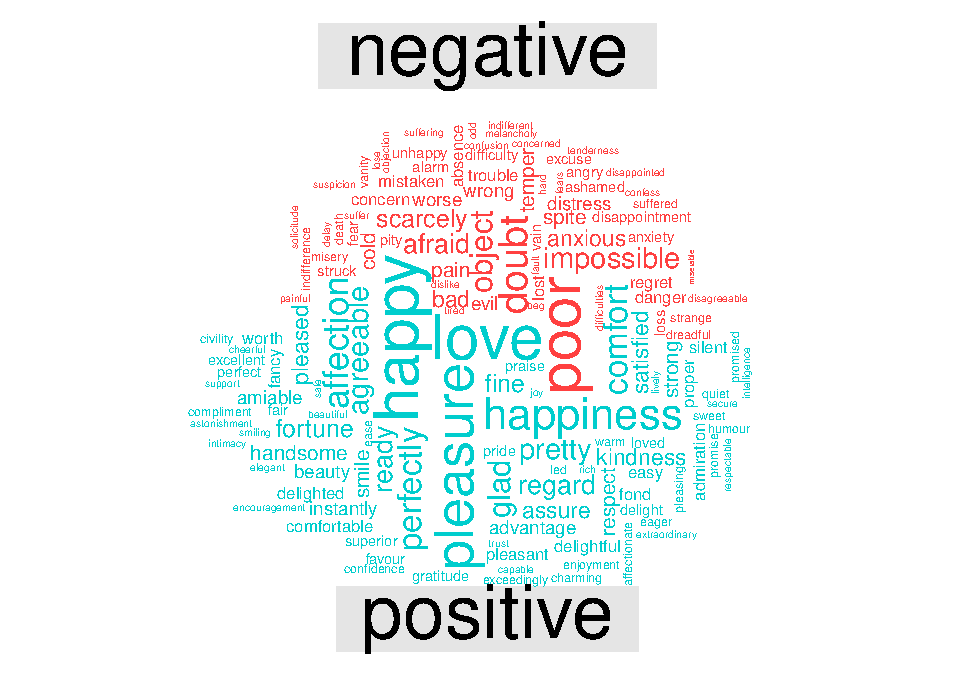
\includegraphics{Week8_files/figure-latex/unnamed-chunk-12-1.pdf}

Syuzhet package

\begin{Shaded}
\begin{Highlighting}[]
\FunctionTok{library}\NormalTok{(zoo)}
\FunctionTok{library}\NormalTok{(syuzhet)}
\end{Highlighting}
\end{Shaded}

One of the more popular specialized sentiment analysis packages.
Available dictionaries: bing, afinn, nrc, syuzhet Getting a particular
novel as a single character string, ready for syuzhet analysis. Let's
first load the Austen novels from scratch, so that we have a clean slate

\begin{Shaded}
\begin{Highlighting}[]
\NormalTok{austen\_tidy\_texts }\OtherTok{\textless{}{-}} \FunctionTok{gutenberg\_download}\NormalTok{(austen\_meta}\SpecialCharTok{$}\NormalTok{gutenberg\_id,}
                                        \AttributeTok{meta\_fields =} \StringTok{"title"}\NormalTok{)}

\NormalTok{persuasion\_tidy }\OtherTok{\textless{}{-}}\NormalTok{ austen\_tidy\_texts }\SpecialCharTok{\%\textgreater{}\%} \CommentTok{\#this extracts only the text of Persuasion}
  \FunctionTok{filter}\NormalTok{(title }\SpecialCharTok{==} \StringTok{"Persuasion"}\NormalTok{)}

\NormalTok{persuasion\_string }\OtherTok{\textless{}{-}} \FunctionTok{paste}\NormalTok{(persuasion\_tidy}\SpecialCharTok{$}\NormalTok{text, }\AttributeTok{collapse =} \StringTok{" "}\NormalTok{) }\CommentTok{\# Extracting the text column as }
\CommentTok{\#character string}

\NormalTok{persuasion\_sentences }\OtherTok{\textless{}{-}} \FunctionTok{tolower}\NormalTok{(}\FunctionTok{get\_sentences}\NormalTok{(persuasion\_string)) }\CommentTok{\# Extract sentences \& lowercase}

\NormalTok{persuasion\_sentiment }\OtherTok{\textless{}{-}} \FunctionTok{get\_sentiment}\NormalTok{(persuasion\_sentences, }\AttributeTok{method =} \StringTok{"syuzhet"}\NormalTok{) }\CommentTok{\# Get sentiment for each sentence}
\end{Highlighting}
\end{Shaded}

\begin{Shaded}
\begin{Highlighting}[]
\NormalTok{pwdw }\OtherTok{\textless{}{-}} \FunctionTok{round}\NormalTok{(}\FunctionTok{length}\NormalTok{(persuasion\_sentiment)}\SpecialCharTok{*}\NormalTok{.}\DecValTok{1}\NormalTok{) }
\NormalTok{persuasion\_rolled }\OtherTok{\textless{}{-}} \FunctionTok{rollmean}\NormalTok{(persuasion\_sentiment, }\AttributeTok{k=}\NormalTok{pwdw) }\CommentTok{\#moving/rolling average (1/10 window)}
\NormalTok{persuasion\_list }\OtherTok{\textless{}{-}} \FunctionTok{rescale\_x\_2}\NormalTok{(persuasion\_rolled) }\CommentTok{\# rescaled so another novel can be compared}
\FunctionTok{plot}\NormalTok{(persuasion\_list}\SpecialCharTok{$}\NormalTok{x, }
\NormalTok{     persuasion\_list}\SpecialCharTok{$}\NormalTok{z, }
     \AttributeTok{type=}\StringTok{"l"}\NormalTok{, }\CommentTok{\# line plot}
     \AttributeTok{main =}\StringTok{"Persuasion Plot Trajectory"}\NormalTok{, }\CommentTok{\# title}
     \AttributeTok{col=}\StringTok{"black"}\NormalTok{, }\CommentTok{\# color of the line}
     \AttributeTok{xlab=}\StringTok{"Narrative Time"}\NormalTok{, }\CommentTok{\# }
     \AttributeTok{ylab=}\StringTok{"Emotional Valence"}\NormalTok{) }\CommentTok{\#This is almost perfect, but it\textquotesingle{}s not smoothed out just right. }
\end{Highlighting}
\end{Shaded}

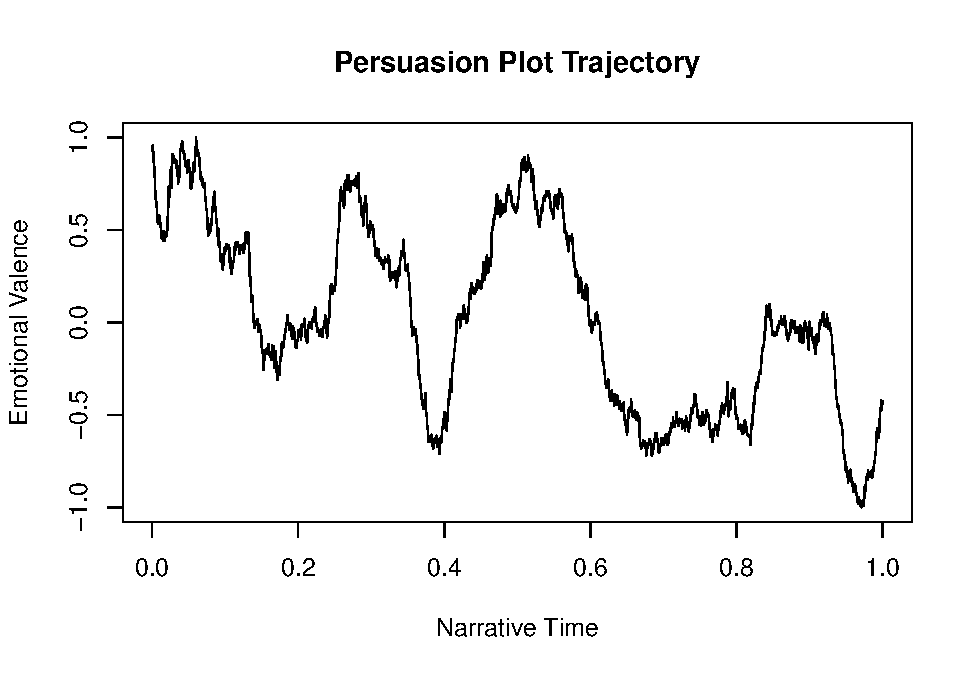
\includegraphics{Week8_files/figure-latex/unnamed-chunk-15-1.pdf}

\begin{Shaded}
\begin{Highlighting}[]
\NormalTok{persuasion\_sample }\OtherTok{\textless{}{-}} \FunctionTok{seq}\NormalTok{(}\DecValTok{1}\NormalTok{, }\FunctionTok{length}\NormalTok{(persuasion\_list}\SpecialCharTok{$}\NormalTok{x),  }
                         \AttributeTok{by=}\FunctionTok{round}\NormalTok{(}\FunctionTok{length}\NormalTok{(persuasion\_list}\SpecialCharTok{$}\NormalTok{x)}\SpecialCharTok{/}\DecValTok{100}\NormalTok{)) }\CommentTok{\# Taking 100 equal chunks of the text}
\FunctionTok{plot}\NormalTok{(persuasion\_list}\SpecialCharTok{$}\NormalTok{x[persuasion\_sample], }
\NormalTok{     persuasion\_list}\SpecialCharTok{$}\NormalTok{z[persuasion\_sample],}
     \AttributeTok{type=}\StringTok{"l"}\NormalTok{, }\CommentTok{\# line plot}
     \AttributeTok{lwd =} \DecValTok{2}\NormalTok{, }\CommentTok{\# line width}
     \AttributeTok{main =} \StringTok{"Persuasion Plot Trajectory"}\NormalTok{,}\CommentTok{\# title}
     \AttributeTok{col=}\StringTok{"black"}\NormalTok{, }\CommentTok{\# color of the line}
     \AttributeTok{xlab=}\StringTok{"Narrative Time"}\NormalTok{,}\CommentTok{\#x axis name}
     \AttributeTok{ylab=}\StringTok{"Emotional Valence"}\NormalTok{,}\CommentTok{\#y axis name}
\NormalTok{)}
\end{Highlighting}
\end{Shaded}

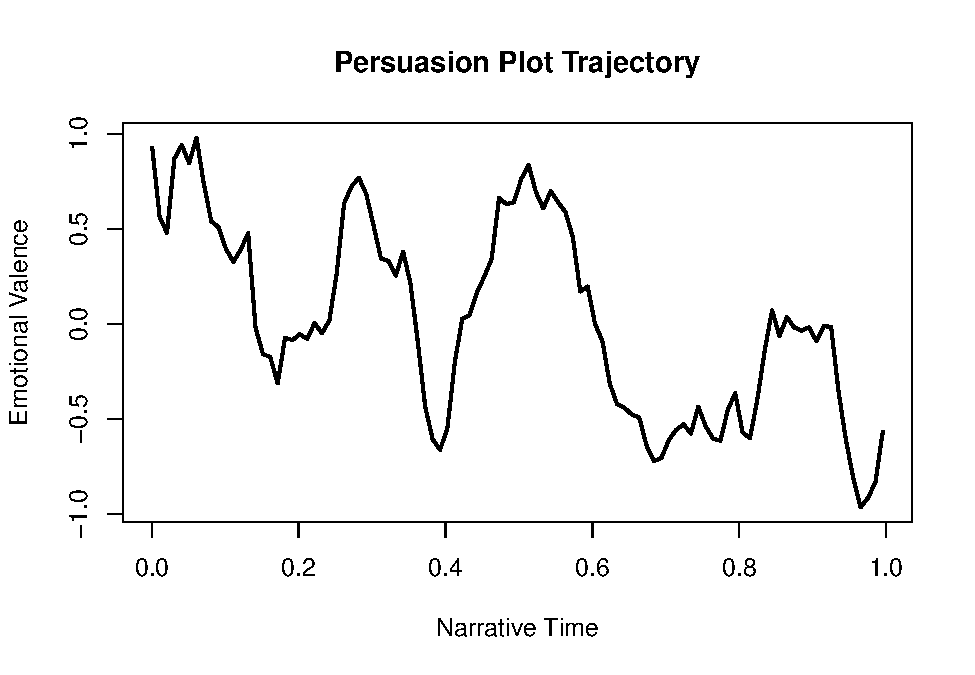
\includegraphics{Week8_files/figure-latex/unnamed-chunk-15-2.pdf}

Package of the week Sentimentr A sentiment analysis package that is more
sophisticated in several ways than both tidytext and

\begin{Shaded}
\begin{Highlighting}[]
\CommentTok{\# syuzhet. Available dictionaries: }
\end{Highlighting}
\end{Shaded}

\begin{Shaded}
\begin{Highlighting}[]
\FunctionTok{library}\NormalTok{(sentimentr)}
\FunctionTok{library}\NormalTok{(magrittr)}

\NormalTok{austen\_sentiment }\OtherTok{\textless{}{-}}\NormalTok{ austen\_tidy\_texts }\SpecialCharTok{\%\textgreater{}\%}  
  \FunctionTok{mutate}\NormalTok{(}\AttributeTok{sentences =} \FunctionTok{get\_sentences}\NormalTok{(text)) }\SpecialCharTok{\%$\%}
  \FunctionTok{sentiment\_by}\NormalTok{(sentences, title)}

\NormalTok{hardy\_sentiment }\OtherTok{\textless{}{-}}\NormalTok{ hardy\_tidy\_texts }\SpecialCharTok{\%\textgreater{}\%} 
  \FunctionTok{mutate}\NormalTok{(}\AttributeTok{sentences =} \FunctionTok{get\_sentences}\NormalTok{(text)) }\SpecialCharTok{\%$\%}
  \FunctionTok{sentiment\_by}\NormalTok{(sentences, title)}

\NormalTok{author\_column }\OtherTok{\textless{}{-}} \FunctionTok{factor}\NormalTok{(}\FunctionTok{c}\NormalTok{(}\StringTok{"Austen"}\NormalTok{, }\StringTok{"Austen"}\NormalTok{,}\StringTok{"Austen"}\NormalTok{,}\StringTok{"Austen"}\NormalTok{,}\StringTok{"Austen"}\NormalTok{,}\StringTok{"Austen"}\NormalTok{,}
                          \StringTok{"Austen"}\NormalTok{,}\StringTok{"Austen"}\NormalTok{,}\StringTok{"Hardy"}\NormalTok{, }\StringTok{"Hardy"}\NormalTok{,}\StringTok{"Hardy"}\NormalTok{,}\StringTok{"Hardy"}\NormalTok{,}
                          \StringTok{"Hardy"}\NormalTok{,}\StringTok{"Hardy"}\NormalTok{,}\StringTok{"Hardy"}\NormalTok{,}\StringTok{"Hardy"}\NormalTok{,}\StringTok{"Hardy"}\NormalTok{,}\StringTok{"Hardy"}\NormalTok{,}
                          \StringTok{"Hardy"}\NormalTok{,}\StringTok{"Hardy"}\NormalTok{,}\StringTok{"Hardy"}\NormalTok{,}\StringTok{"Hardy"}\NormalTok{,}\StringTok{"Hardy"}\NormalTok{))}
\end{Highlighting}
\end{Shaded}

Combining the austen and hardy sentiment dataframes

\begin{Shaded}
\begin{Highlighting}[]
\NormalTok{hardy\_vs\_austen }\OtherTok{\textless{}{-}} \FunctionTok{rbind}\NormalTok{(austen\_sentiment, hardy\_sentiment)}
\end{Highlighting}
\end{Shaded}

Adding the author column, which is already a factor vector

\begin{Shaded}
\begin{Highlighting}[]
\NormalTok{hardy\_vs\_austen }\OtherTok{\textless{}{-}}\NormalTok{ hardy\_vs\_austen }\SpecialCharTok{\%\textgreater{}\%} 
  \FunctionTok{cbind}\NormalTok{(author\_column)}
\end{Highlighting}
\end{Shaded}

The resulting dataframe is an ideal use case for a boxplot/violin plot
visualization. Let's use the ggstatsplot package we used in week 5.

\begin{Shaded}
\begin{Highlighting}[]
\FunctionTok{library}\NormalTok{(ggstatsplot)}
\end{Highlighting}
\end{Shaded}

Final visualization

\begin{Shaded}
\begin{Highlighting}[]
\FunctionTok{options}\NormalTok{(}\AttributeTok{scipen =} \DecValTok{10000}\NormalTok{)}

\NormalTok{hardy\_vs\_austen\_plot }\OtherTok{\textless{}{-}} \FunctionTok{ggbetweenstats}\NormalTok{( }
  \AttributeTok{data =}\NormalTok{ hardy\_vs\_austen, }\CommentTok{\# data}
  \AttributeTok{x =}\NormalTok{ author\_column, }\CommentTok{\# data for x axis}
  \AttributeTok{y =}\NormalTok{ ave\_sentiment, }\CommentTok{\# data for y axis}
  \AttributeTok{title =} \StringTok{"Comparison of the mean sentiment of Hardy\textquotesingle{}s and Austen\textquotesingle{}s novels"}\NormalTok{, }\CommentTok{\# Title}
  \AttributeTok{xlab =} \StringTok{"Author"}\NormalTok{, }\CommentTok{\# x axis label}
  \AttributeTok{ylab =} \StringTok{"Sentiment"} \CommentTok{\# y axis label}
\NormalTok{)}
\NormalTok{hardy\_vs\_austen\_plot}
\end{Highlighting}
\end{Shaded}

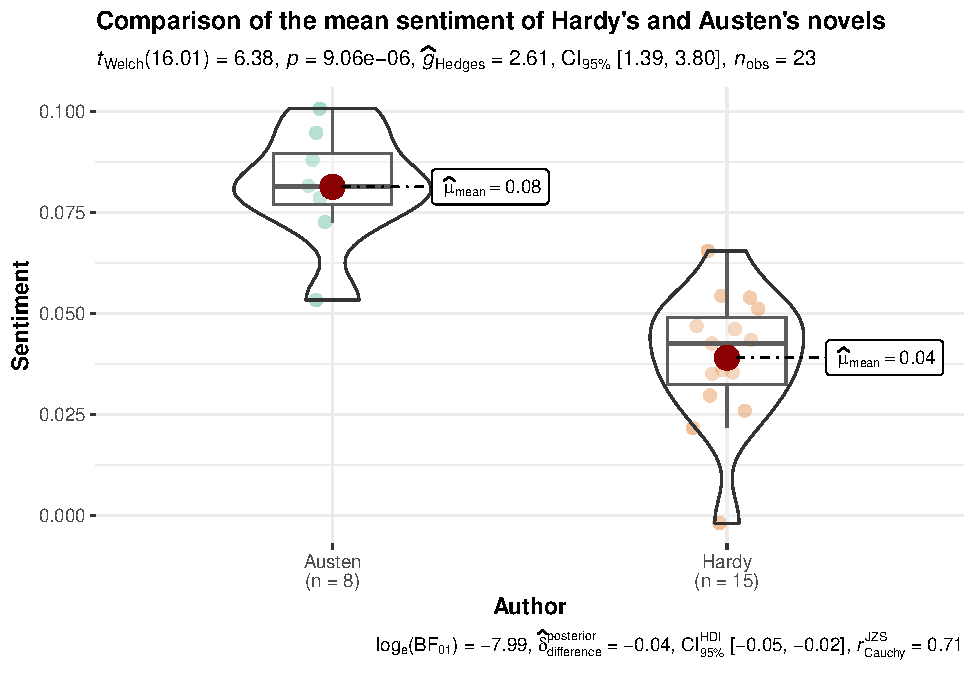
\includegraphics{Week8_files/figure-latex/unnamed-chunk-21-1.pdf}

\end{document}
